%!TEX root = ../dissertation.tex

\chapter{Architecture}
\label{chapter:architecture}
As previously mentioned, the OpenFlow specification provides mechanisms for resilience and load balancing across multiple \gls{SDN} controller instances.
These mechanisms however require complex mechanisms of inter-instance coordination and cumbersome configuration tasks on the OpenFlow switche(es).\\
%
The basic principle of the proposed architecture is to replace the \gls{SDN} controller by a cluster of \gls{SDN} controllers, which keep a consistent \gls{MIB} between them.
Any individual controller in the cluster is able to manage any OpenFlow device in the same network domain.
Load balance between controllers is provided by introducing southbound and northbound request routers, which may themselves be replicated for redundancy proposes.
The proposed solution enables controllers to be dynamically added to or removed from the cluster without network disruption or OpenFlow switch reconfiguration, therefore providing an \emph{elastic} structure.
%
\section{Elastic SDN controller cluster}
\label{section:SDN-controller-cluster}
OpenFlow allows for an OpenFlow switch to be connected to several \gls{SDN} controllers simultaneously, however, the latter are expected to have some sort of coordination between them in order to achieve load balancing and instance failure resiliency, which is achieved by exposing eastbound/westbound \glspl{API} to be consumed by neighboring controllers within the same management domain.
%
Having the instances coordinated with each other and keep consistent states in a distributed environment requires therefore a \gls{SDN} controller cluster and configures an architecture such that of figure \ref{fig:sdn_simple_clustering}.\\
%
\begin{figure}
	\centering
	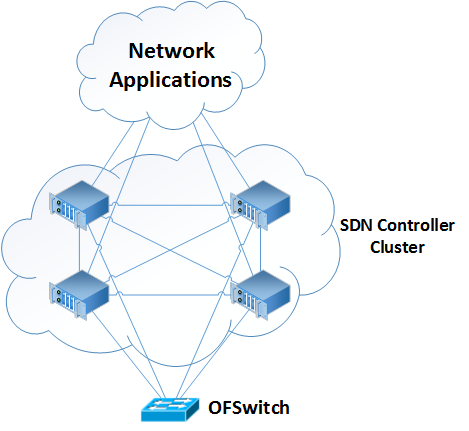
\includegraphics[scale=0.50]{sdn_simple_clustering}
	\caption{OpenFlow SDN controller clustering}
	\label{fig:sdn_simple_clustering}
\end{figure}
%
\gls{SDN} cluster instances must then provide eastbound/westbound \glspl{API}s that allow for cluster membership operations.
The resulting cluster should support key aspects of the \gls{SDN} controller component, such as keep a global view and management scope.
Because the goal is to perform load balancing between all instances, each instance will be actively managing any given number of OpenFlow switches in the same management domain, and therefore the network state is distributed in nature.
In order to improve scalability and resiliency, new \gls{SDN} controller instances can be added, and removed on demand from the cluster without requiring any reconfiguration or service interruption.\\
%
To that extent, when a new \gls{SDN} controller instance is initialized it must advertise itself to all existing \gls{SDN} controller instances, forming a cluster if only one other instance existed prior to the advertisement or otherwise joining the existing cluster.
In order for this to be accomplished either the newly instantiated \gls{SDN} controller would require to have prior knowledge of all existing instances or instead some mechanism of peer instance discovery.
Peer instance discovery offers a mechanism much closer to the zero-configuration goal that this architecture aims at.
The discovery mechanism considered is that of \emph{group communication}, which is itself a form of \emph{indirect communication}, in which the sender is not aware of the receivers and thus instead of sending the message to a specific receiver it sends the message to a group, which will then have the message delivered to all members of said group\cite{PADI}.\\
Upon joining a cluster, regardless if new or existing, the joining instance(s) must then synchronize its \gls{MIB} with any other peer instance, from which point on it will proceed to process updates from other peers.
The \gls{SDN} controller instance cluster registration process is defined in figure \ref{fig:cluster_registration_process}, and the set of messages for cluster membership in table \ref{table:cluster-message-spec}\\
%
\begin{figure}
	\centering
	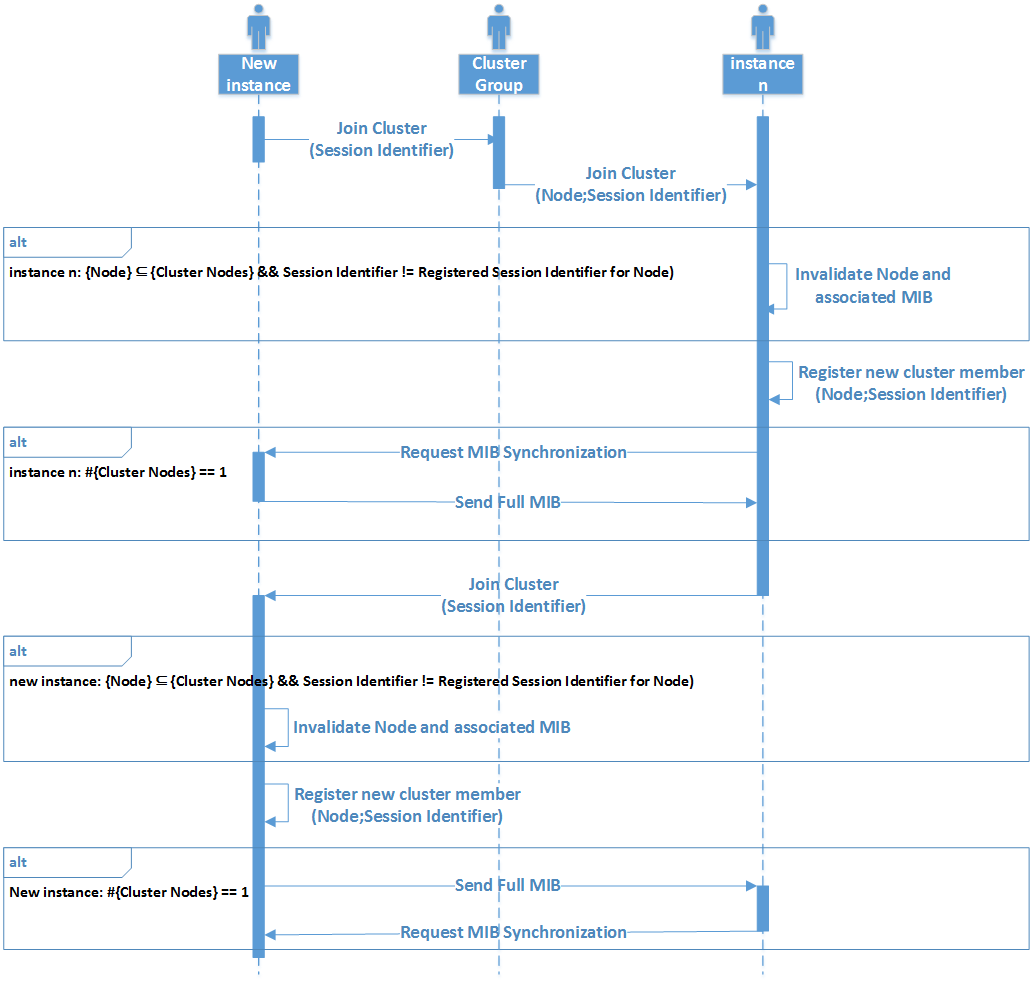
\includegraphics[scale=0.60]{cluster_member_registration}
	\caption{SDN elastic cluster membership registration}
	\label{fig:cluster_registration_process}
\end{figure}
%
Because \gls{SDN} controller instances are prone to failure due to software, hardware or network failures at any given point in time and without being able to notify its peers, it is important to provide a mechanism that makes every cluster member aware of peers state.
As such, two mechanism have been defined for instance failure detection: session identifiers and periodic health checks.\\
\gls{SDN} controller instances must generate a unique session identifier when initializing itself, which will then serve as an identifying key for cluster members, and therefore must be included in every message exchanged with peering instances.
When a \gls{SDN} controller instance $\alpha$ receives a message from a peer instance $\beta$ which is identified by session identifier $\upsilon$, $\alpha$ must validate that the membership key $\kappa$ it holds for peer $\beta$ has not changed ($\kappa$=$\upsilon$) before processing the message.
Should the session identifier have changed ($\kappa$$\neq$$\upsilon$), $\alpha$ must invalidate all \gls{MIB} registries it held associated with peer $\beta$.\\
In order to ensure fast failure detection and quickly invalidate any \gls{MIB} registry that might lead to erroneous forwarding decisions, all \gls{SDN} controller instances participating in a cluster must send periodic (every $\Delta$ seconds) \gls{Keepalive} notifications to its peers.
Should an instance $\alpha$ fail to receive three consecutive \gls{Keepalive} notifications (3$\Delta$ seconds) from a peer instance $\beta$, then $\alpha$ must assume that $\beta$ is no longer available and therefore render all \gls{MIB} entries associated with $\beta$ invalid.\\
%
In order to maintain the aforementioned behavior, active instances must issue cluster membership and \gls{MIB} updates to their cluster peers and be prepared to receive membership and update their own \gls{MIB} with updates issued by their peers.
The propagation of \gls{MIB} updates must be triggered for every network event detected by a given instance.
The minimum set of cluster membership and \gls{MIB} update messages and associated events, along with which instances must be notified, are specified in table \ref{table:cluster-message-spec}.
%
\begin{table}[h!]
	\begin{center}
		\rowcolors{2}{EvenRowColor}{OddRowColor}
		\begin{tabular}{ | l | p{3,5cm} | p{6cm} | p{1,5cm} | }
			\rowcolor{HeaderRowColor}
			\hline
			\textbf{Scope} & \textbf{Message} & \textbf{Event} & \textbf{Target}\\
			\hline
			Cluster membership & Join cluster & New \gls{SDN} controller instance created and requesting to join the existing cluster & cluster\\
			\hline
			Cluster membership & Leave cluster & \gls{SDN} controller instance shutting down and requesting to leave the cluster & cluster\\
			\hline
			Cluster membership & Instance health & \gls{SDN} controller instance periodic health report & cluster\\
			\hline
			Cluster membership & Full Synchronization Request & \gls{SDN} controller instance requesting a full \gls{MIB} update & specific instance\\
			\hline
			Cluster membership & Full Synchronization Reply & \gls{SDN} controller instance replying to a full \gls{MIB} update & specific instance\\
			\hline
			\gls{MIB} update & Add Switch & New OpenFlow switch connected to an instance & cluster\\
			\hline
			\gls{MIB} update & Remove Switch & OpenFlow switch disconnected from an instance & cluster\\
			\hline
			\gls{MIB} update & Add Host & New host connected to the network & cluster\\
			\hline
			\gls{MIB} update & Remove Host & Host disconnected from the network & cluster\\
			\hline
			\gls{MIB} update & Add Inter-switch link & New neighbor adjacency detected & cluster\\
			\hline
			\gls{MIB} update & Remove Inter-switch link & Neighbor adjacency lost & cluster\\
			\hline
		\end{tabular}
		\caption{Cluster messages}
		\label{table:cluster-message-spec}
	\end{center}
\end{table}
%
When a \gls{SDN} cluster instance propagates updates to other peer instances, it must guarantee \emph{causal consistency}, thus ensuring that any dependencies between updates is met.
Causal consistency ensures that messages send by an instance $\alpha$ are seen by every other instance receiving them in the exact same order that they where sent by $\alpha$, thus guaranteeing \emph{potencial causal ordering} of events throughout the cluster \cite{PADI}.
This property is crucial to maintain the integrity of the distributed data model, as it guarantees that scenarios such as adding an inter-switch link before adding the switches themselves do not happen.\\
%
This architecture allows for coordination between \gls{SDN} controller instances, providing each instance with a global view of the network regardlessly of which network node(s) it manages.
This approach, however, still requires that every OpenFlow switch within the management domain be reconfigured every time an \gls{SDN} controller instance is added to or removed from the \gls{SDN} controller cluster, which takes us back to a manual, decentralized and vendor-specific network management model.\\
%
\section{Request Router}
\label{section:request-router}
% existing solutions
The mechanism provided by OpenFlow to load balance between clustered \gls{SDN} controller instances and inherently provide resilience requires one of the following:
\begin{enumerate}
	\item OpenFlow switches are configured with all the ip addresses of all the controller instances (and then either let Master/Slave role election occur or have the controller implementation extended such that multiple instances in Equal role can coordinate between themselves which instance will process which event)
	\item The network is partitioned such that different subsets of network are controlled by different controllers as depicted in figure \ref{fig:static_controller_distribution}
\end{enumerate}
%
\begin{figure}
	\centering
	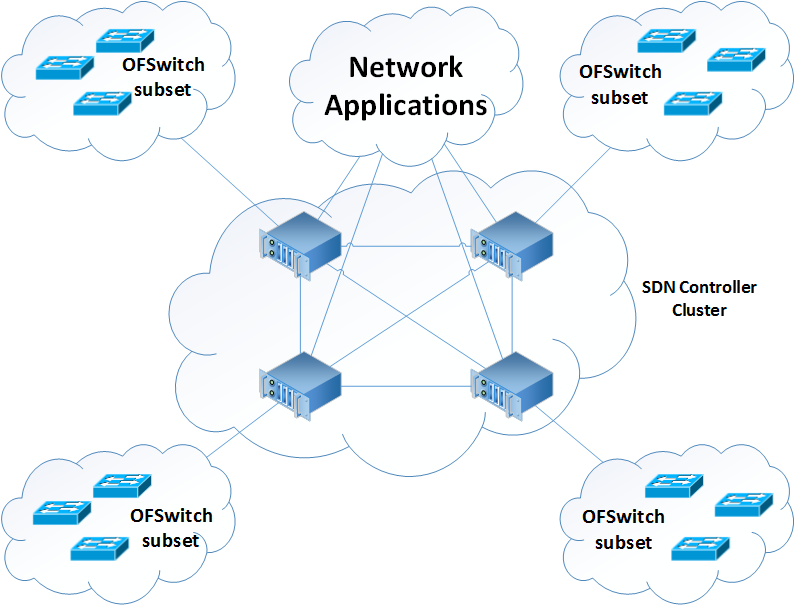
\includegraphics[scale=0.35]{static_controller_distribution}
	\caption{Static SDN Controller load balancing}
	\label{fig:static_controller_distribution}
\end{figure}
%
% Problems with existing solutions
The first approach adds a considerable amount of complexity both to the OpenFlow switch configuration and to the controller implementation, providing however the basis for equitable load balancing and controller resiliency.
The second has the advantage of removing complexity both from the OpenFlow switches and the controller implementation, but it is still suboptimal as it does not guarantee equal load balancing across controller instances. In fact, a subset $\alpha$ of OpenFlow switches may process more traffic flows than a subset $\beta$, resulting in a higher computational load on the instance controlling subset $\alpha$ when compared to the instance controlling subset $\beta$.\\
%
% Requirements
In order to provide a solution that keeps the advantages and discards the disadvantages of both approaches, it is then necessary for the existence of a mechanism that transparently assigns the less-loaded instance to an OpenFlow switch - a load balancing component.
This new component, the \emph{request router}, must be completely transparent to all three components of the \gls{SDN} architecture, while providing load balance between \gls{SDN} controller instances without compromising infrastructure resiliency.\\
%
% Request Router Overview
The request router encapsulates all the controller instances as a single virtual instance from the OpenFlow switches and network applications point of view, by logically sitting between the \gls{SDN} controller instances and the OpenFlow switches and having the OpenFlow switches connect to a request router instance instead.
The request router is then responsible to determine which is the best \gls{SDN} controller instance to handle the OpenFlow switch and forward the request to that instance.\\
%
% Controller instance discovery
To be able to forward connections to \gls{SDN} controller instances, it is necessary for the request router to be aware of existing \gls{SDN} controller instances so that the logical topology described in figure \ref{fig:distributed_controller_rr} can be achieved.
This can be attained simply by having the request router instances joining the communication group described in section \ref{section:SDN-controller-cluster} and listening for the cluster membership messages described in table \ref{table:cluster-message-spec}.
The same \gls{Keepalive} mechanism described in section \ref{section:SDN-controller-cluster} must also be implemented on the request router in order for request routers to also detect failing \gls{SDN} controller instances.\\
%
\begin{figure}
	\centering
	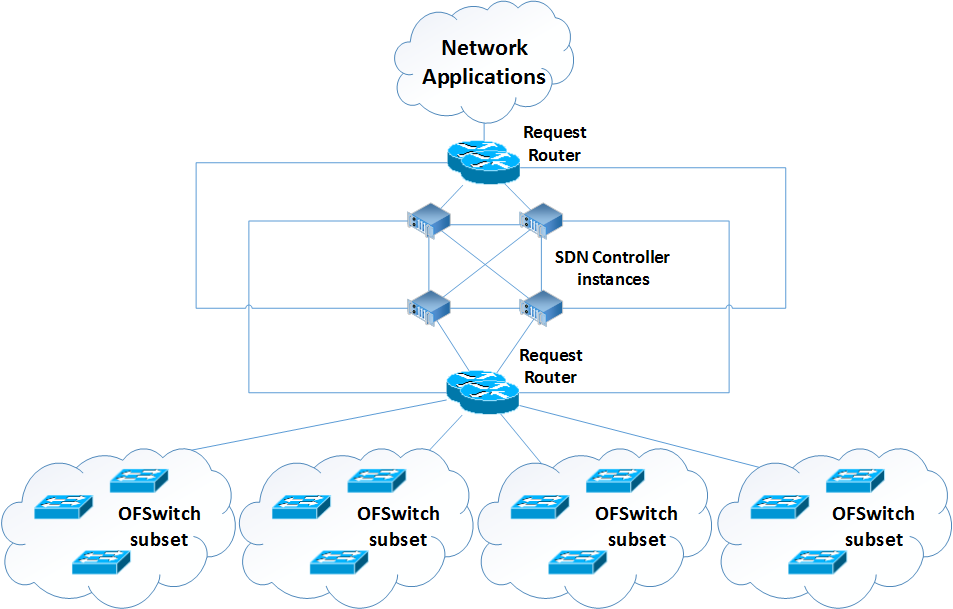
\includegraphics[scale=0.45]{distributed_controller_rr}
	\caption{Request Router integration with \gls{SDN} controller instances}
	\label{fig:distributed_controller_rr}
\end{figure}
%
% Redundancy (failure+LB)
In order to maintain infrastructure resiliency, it is imperative that the execution of the load balance function does not affect the connections between OpenFlow switches and \gls{SDN} controller instances and that a failure of any given request router instance does not have impact on the load balancing service.
The request router then must implement a clustering mechanism that allows the existence of several request router instances, in which active OpenFlow switch management connections are processed by any available request router instance, thus load balancing the connections between themselves so that request router instances do not become overloaded, and where any request router instance $\alpha$ can take over the tasks performed by instance $\beta$ should $\beta$ fail.\\
% Load Balancing the RR - Anycast
To ensure that OpenFlow switch management connections to \gls{SDN} controller instances are load balanced between available request routers without requiring reconfiguration of the OpenFlow switches, request router instances implement the \gls{anycast} communication paradigm.
By implementing \gls{anycast}, OpenFlow switches will connect to whichever request router instance is logically closer to them, and thus providing a mechanism to load balance OpenFlow switch management connections between request router instances.
% Local and Global LB
Because large network topologies often span over several geographical locations and OpenFlow switches will connect to whichever request router is closer to them, request routers instances in the same request router cluster are allowed to have different forwarding rules so that OpenFlow switch management connections can be forwarded to the closest least-loaded or to the globally least-loaded \gls{SDN} cluster instance according to the network administrators preferences, thus resulting the in topology depicted in figure \ref{fig:Amorphous}.\\
%
\begin{figure}
	\centering
	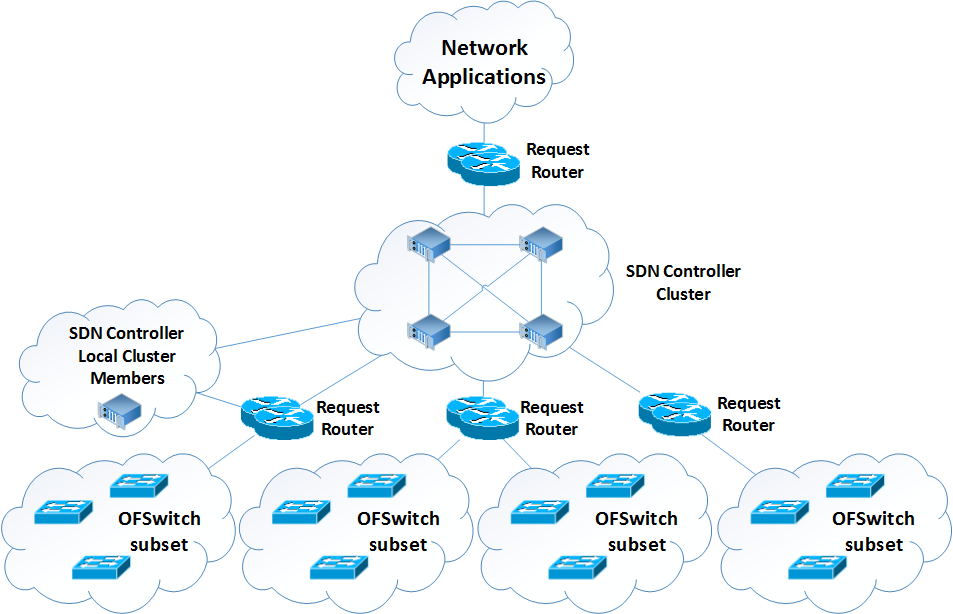
\includegraphics[scale=0.50]{Amorphous}
	\caption{Logical overview of the proposed architecture}
	\label{fig:Amorphous}
\end{figure}
%
%
\begin{figure}
	\centering
	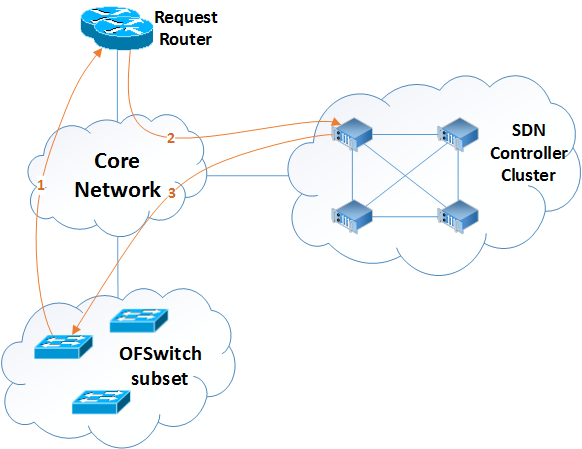
\includegraphics[scale=0.50]{rr_message_flow}
	\caption{OpenFlow switch management connections load balanced by Request Routers}
	\label{fig:rr_message_flow}
\end{figure}
%
% How it works
As mentioned in chapter \ref*{chapter:state-of-the-art} section \ref{section:openflow}, OpenFlow switches are required to maintain active \gls{TCP} or \gls{TLS} connections with the configured \gls{SDN} controller(s).
Since we are now considering the topology represented in figure \ref{fig:Amorphous} and the description, we now consider that the all OpenFlow switches are configured to connect exclusively to the request router cluster, which in turn will forward the connection to an \gls{SDN} controller instance.
The \gls{SDN} controller instance then replies directly to the OpenFlow switch, as portrayed in figure \ref{fig:rr_message_flow}.
Having this behavior as opposed to having the \gls{SDN} controller instance reply back to the request router instance improves both performance and scalability as the latency for the response packets will be lower and it removes computational load from the request router instances, thus allowing them to handle more request packets.\\
Because both \gls{TCP} and \gls{TLS} (which uses \gls{TCP} as its transport layer protocol\cite{rfc5246}) are connection oriented, request router instances must always forward packets coming from an OpenFlow switch to the same \gls{SDN} controller instance.
Therefore, the request router must implement a deterministic destination selection for all packets coming from the same OpenFlow switch, such that any request router instance will forward the packets from switch $\alpha$ to the exact same \gls{SDN} controller instance $\beta$.
Should $\beta$ become unavailable then request router instances are required to stop forwarding packets to $\beta$ and assign a new \gls{SDN} controller instance $\upsilon$ and forward all packets from $\alpha$ to $\upsilon$.
